\documentclass[12pt]{article}
%\usepackage{url}

\setlength{\parindent}{0in}
\setlength{\parskip}{0.1in}
\usepackage{graphicx}
\usepackage{fullpage}

\begin{document}
\begin{center}
{ \Large Department of Physics \& Astronomy \\ \medskip Austen Report Response \\ \medskip May 2016}
\end{center}
\section{Implications}

\subsection{Demand}

{\bf External Demand:}  We have the second highest demand in college.
We are good here.


{\bf Internal Demand:} Percent of graduates who complete each major.

This is currently low but we expect it to increase.

\subsection{Cost}

Our cost per major is high, but we have failed to understand why we are higher than other science departments.  
We are in the process of trying to independently reproduce the cost analysis estimates so that we
can better understand the factors that contribute to our cost.

Our overall cost looks very good - our total cost, total revenue and total margin presents a different picture.  

Department consistently brings in grants.  

\subsection{Yield}

Number of enrolled majors divided by number of external inquiries.  Our yield is low, which indicates that we have 
the potetial for continued growth.  We are assuming that many of the external inquiries are for engineering.  The fact that 
we don't have engineering.  

\section{Factors and Actions}

We are looking into a new major that is applied physics or pre-engineering.

need more space if we are to grow.

we will improve our website.  the college needs to improve its website as well.

We have maintained an active role in open houses.  We will work with admissions to increase
contact with prospective students in the late fall and spring to better communicate the strengths of
our department and program.


We look forward to working with new marketing department.  market programs in physics and astronomy.

spending 50\% of operating budget is spent on program.

1/3 of people are teaching.  2/3 non teaching.  

national marketing effort to match the growing national reputation of our department.


\section{Reflection on Austen Report}

Our combination of demand, cost and yield is unique; we have high demand, high cost, and low yield. 
We interpret high demand and low yield to mean that we have potential to continue to increase the number of majors.  We have already increased our overall number of majors during the 2013-2015 period (see Fig. \ref{nmajors}).
\begin{figure}[h]
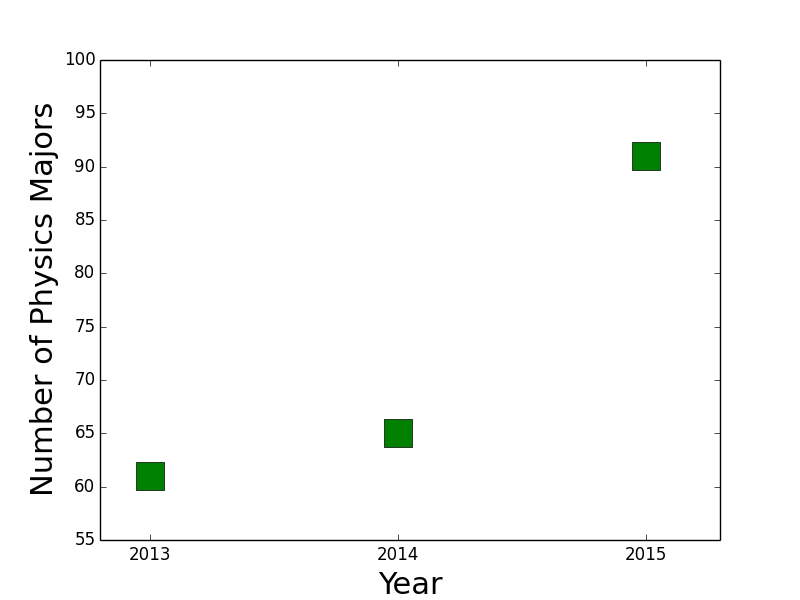
\includegraphics[width=.85\textwidth]{Nmajors_year.png}
\caption{Number of physics majors vs. year.}
\label{nmajors}
\end{figure}


We have already increased recruiting efforts.  Need to see how changes impact our program.

We can decrease cost per
student credit hour by increasing enrollment.  

% \begin{table}
% \begin{tabular}{lrrrr}
%   Dept & Ave class size & SCH & cost & total rev & total margin \\
% \hline
% math &18 &  6915 & 1978206 & 2718580 & 27 \\
% physics &21 &  5827 & 2013888 & 2739528 & 26 \\
% chemistry & 18 &6880 & 2478207 & 2877539 & 14 \\
% \end{tabular}
% \end{table}

% john's figure from ipeds

\begin{figure}[h]
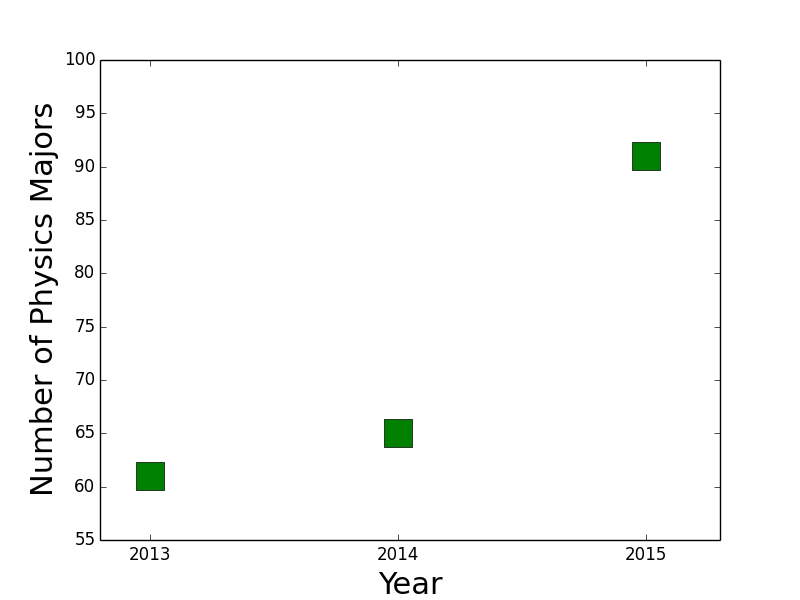
\includegraphics[width=.85\textwidth]{Nmajors_year.png}
\caption{Number of faculty, staff, and administrators vs. year.}
\label{nmajors}
\end{figure}

\end{document}